\item \textbf{{[}RVHS/PRELIM/9597/2017/P1/Q5{]} }

\textbf{Grocery Store Manager }

The grocery shop in the neighborhood ask your help to create an application
to manage the grocery store. 

First, you are tasked to work on an object-oriented solution to store
all the grocery details. The \texttt{title} of the grocery item, \texttt{cost},
\texttt{price} and \texttt{stock} of each grocery is recorded. Besides
the normal groceries, the shop identifies three unique types of grocery
too, namely:
\begin{itemize}
\item Electrical Appliance: there is a need to indicate the \texttt{power}
of the product to understand its energy consumption rate.
\item Cigarette: it is important to track the \texttt{nicotine content}
of various kinds of cigarette.
\item Alcohol: there are distinct \texttt{types} of alcohols such as wine
or beer. 
\end{itemize}
Below is an UML class diagram for your reference. 

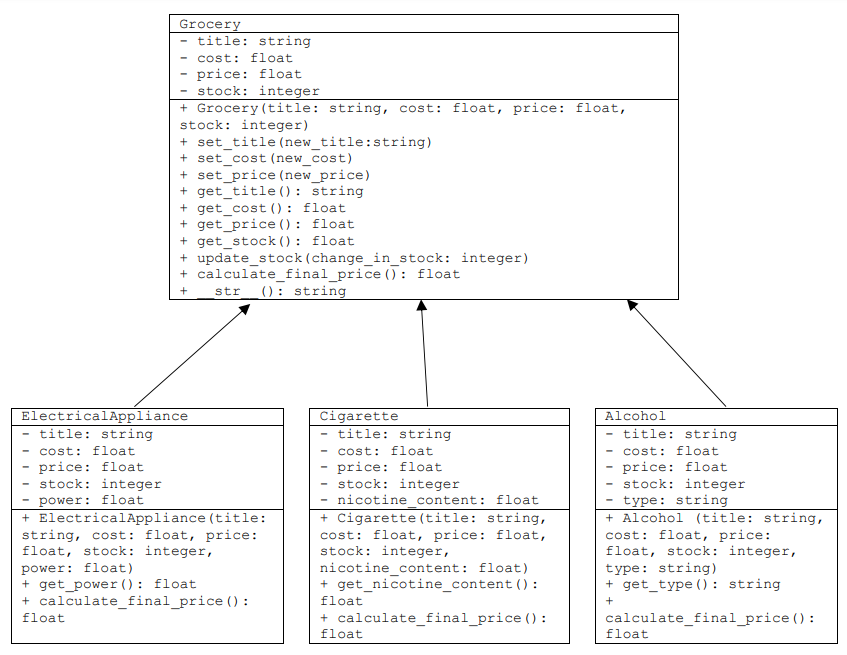
\includegraphics[width=0.65\paperwidth]{C:/Users/Admin/Desktop/Github/question_bank/LyX/static/img/9597-RVHS-2017-P1-Q5-1}

\subsection*{Task 5.1}

Implement the classes of \texttt{Grocery}, \texttt{ElectricalAppliance},
\texttt{Cigarette} and \texttt{Alcohol} with object-oriented programming.

\subsection*{Evidence 18}

Program Code for four classes. \hfill{}{[}7{]}

\subsection*{Task 5.2 }

In country S, purchasing all groceries will incur a 7\% Goods and
Services Tax(GST). 

To promote healthy living, additional tax have been imposed to cigarettes
and alcohols: 
\begin{itemize}
\item Cigarette: additional 60\% tax 
\item Wines: additional 50\% tax 
\item Beers: additional 20\% tax 
\end{itemize}
For example: \emph{the price of one packet of \textquotedblleft Yun
Yan\textquotedblright{} cigarette is \$23.00, the final price can
be calculated by: \$23.00 x 160\% x 107\% = \$39.38}

In addition, to support the \textquotedblleft save energy movement\textquotedblright ,
all electrical appliance with a power less than or equals to 10Watt
was set to be sold at 80\% of its original price. 

Implement the function \texttt{calculate\_final\_price()} which includes
the above mentioned tax and promotion into consideration. 

Implement the \texttt{\_\_str\_\_()} function which returns a string
in the following format (You may refer to the \texttt{test\_function\_5\_1()}
to understand the formatting): 

\texttt{Title | Cost | Price | Stock | Final Price }

For example, Yun Yan\textquoteright s cost is \$16.50, price is set
at \$23.00, the current stock is 4 and final price is \$39.38. The
\_\_str\_\_() function should return the following string:

\texttt{Yun Yan | \$ 16.50 | \$ 23.00 | 4 | \$ 39.38}

\subsection*{Evidence 19 }

Program Code for \texttt{calculate\_final\_price()} and \texttt{\_\_str\_\_()}. 

Screenshot showing output of \texttt{test\_function\_5\_1()}. \hfill{}{[}6{]}

\subsection*{Task 5.3}

Implement a class \texttt{StoreManager} which keep track of a list
of grocery items, \texttt{curr\_item\_list}. The \texttt{StoreManager}
should have the following class functions: 
\begin{itemize}
\item \texttt{sell\_item(sold\_item)} \texttt{sold\_item} is a tuple containing
2 elements: the \texttt{title} of the item and the \texttt{quantity}
sold. You may assume the title of item is always valid and the quantity
sold is always smaller than the current stock. 

The function should decrease the current stock of the sold items.
Upon completion, it should print out a string containing the following
information:

\texttt{Title | Unit Price | Quantity Sold | Subtotal}

The function should return a float containing the \texttt{sub\_total}
value.
\item \texttt{sell\_items(sold\_item \_list)} \texttt{sold\_item\_list}
is a list of tuples; each tuple containing the item \texttt{title}
and \texttt{quantity} sold. 

The function should print out a table displaying information for all
sold items in the following format: 

\texttt{Title | Unit Price | Quantity Sold | Subtotal}

The summary should end with a line indicating the overall total value
of items sold in this transaction. 
\item \texttt{stock\_check()} When this function is called, it should check
the list of all grocery items and print out a summary of items with
current stock value below 5. This indicates the need for stocking
up these items soon. A summary table should be printed in the following
format: 

\texttt{Title | Unit Cost | Quantity Left }
\end{itemize}

\subsection*{Evidence 20 }

Program Code for class functions of StoreManager class: 
\begin{itemize}
\item sell\_item \hfill{}{[}3{]}
\item sell\_items \hfill{}{[}2{]}
\item stock\_check \hfill{}{[}2{]}
\end{itemize}
Screenshot showing output of \texttt{test\_function\_5\_2()}.\hfill{}
{[}2{]}